\section{Bài tập 4}
\subsection{Giải xấp xỉ hệ phương trình vi phân bằng phương pháp Euler tường minh}
\subsubsection{Phương pháp Euler tường minh}
\hspace*{0.5cm} {Phương pháp Euler tường minh (Explicit Euler method) là phương pháp đơn giản nhất để giải xấp xỉ hệ phương trình vi phân tổng quát (23).} \\
\hspace*{0.5cm} {Với giá trị $R_0, J_0$ là giá trị của hàm $R(t), J(t)$ tại thời điểm ban đầu $t_0$, giá trị xấp xỉ của $R_{k+1}, J_{k+1}$ tại thời điểm $t_{k+1} = t_0 + h.(k+1)$, với $h$ là bước nhảy thời gian, được tính theo công thức:} 
\begin{align}
    \begin{cases}
        R_{k+1} = R_k + f(t_k, R_k, J_k) * h\\
        J_{k+1} = J_k + g(t_k, R_k, J_k) * h
    \end{cases}
\end{align}
\subsubsection{Nguồn gốc}
\hspace*{0.5cm} {Có nhiều cách để suy ra công thức của phương pháp Euler tường minh.}\\
\hspace*{0.5cm} {Cách thứ nhất là sử dụng khai triển Taylor của hàm $R$ và hàm $J$ tại thời điểm $t_k$:}
\begin{align}
    \begin{cases}
        R(t_{k+1}) = R(t_k + h) = R(t_k) + h.R'(t_k) + \frac{1}{2}h^2R"(t_k) + O(h^3)\\
        J(t_{k+1}) = J(t_k + h) = J(t_k) + h.J'(t_k) + \frac{1}{2}h^2J"(t_k) + O(h^3)
    \end{cases}
\end{align}
\begin{align}
    \Rightarrow
    \begin{cases}
        R(t_{k+1}) = R(t_k) + h.f(t_k, R_k, J_k) + \frac{1}{2}h^2f'(t_k, R_k, J_k) + O(h^3)\\
        J(t_{k+1}) = J(t_k) + h.g(t_k, R_k, J_k) + \frac{1}{2}h^2g'(t_k, R_k, J_k) + O(h^3)
    \end{cases}
\end{align}
\hspace*{0.5cm} {Nếu bỏ qua các số hạng bậc hai và bậc cao hơn, ta sẽ có được hệ phương trình (24), chính là phương pháp Euler tường minh.}\\
\hspace*{0.5cm} {Một cách khác chính là biến đổi thông qua công thức sai phân, với $t_{k+1} = t_k + h$, ta cũng thu được phương pháp Euler:}
\begin{align}
    \begin{cases}
        R(t_{k+1}) \approx R(t_k) + (t_{k+1} - t_k)R'(t_k)\\
        J(t_{k+1}) \approx J(t_k) + (t_{k+1} - t_k)J'(t_k)
    \end{cases}
\end{align}
\begin{align}
    \Rightarrow
    \begin{cases}
        R(t_{k+1}) \approx R(t_k) + hf(t_k, R_k, J_k)\\
        J(t_{k+1}) \approx J(t_k) + hg(t_k, R_k, J_k)
    \end{cases}
\end{align}
\hspace*{0.5cm} {Ngoài ra, ta cũng có thể tích phân phương trình vi phân từ $t_k$ tới $t_k + h$ và áp dụng các định lí cơ bản của tích phân và vi phân để có được:}\\
\hspace*{4cm} {$R(t_k + h) - R(t_k) = \displaystyle\int\limits_{t_k}^{t_k + h}f(
t, R(t), J(t)\;\mathrm{d}t$}\\
\hspace*{0.5cm} {Tính xấp xỉ tích phân trên bằng tổng Riemann trái, ta được:}\\
\hspace*{4cm} {$\displaystyle\int\limits_{t_k}^{t_k + h}f(t, R(t), J(t)\;\mathrm{d}t \approx hf(t_k, R(t_k), J(t_k)$}\\
\hspace*{0.5cm} {Kết hợp cả 2 phương trình, ta suy ra phương pháp Euler. Chứng minh tương tự với hàm $J(t)$.}
\subsubsection{Sai số cắt ngắn cục bộ (Local Truncation Error - LTE)}
\hspace*{0.5cm} {Theo phương pháp Euler tường minh đã được đề cập ở phần trên, giá trị xấp xỉ $R_1$, $J_1$ tại thời điểm $t_1 = t_0 + h$, được tính bằng:}
\begin{align}
    \begin{cases}
        R_1 = R_0 + f(t_0, R_0, J_0) * h\\
        J_1 = J_0 + g(t_0, R_0, J_0) * h
    \end{cases}
\end{align}
\hspace*{0.5cm} {"Sai số cắt ngắn cục bộ" của phương pháp Euler là sai số trong 1 bước duy nhất. Nó là khoảng cách giữa kết quả xấp xỉ sau 1 bước $R_1, J_1$ và kết quả chính xác $R(t_1), J(t_1)$ tại thời điểm $t_1 = t_0 + h$. Đối với hệ phương trình vi phân, "sai số cắt ngắn cục bộ" được tính bởi công thức: }\\
\hspace*{4cm} {$E(t_1) = \sqrt{[R(t_1) - R_1]^2 + [J(t_1) - J_1]^2}$}\\
\hspace*{0.5cm} {Với $t_1 = t_0 + h$, áp dụng khai triển Taylor đối với $R(t_1)$ và $J(t_1)$, ta có:}
\begin{align}
    \begin{cases}
        R(t_1) = R(t_0 + h) = R(t_0) + h.R'(t_0) + \frac{1}{2}h^2R"(t_0) + O(h^3)\\
        J(t_1) = J(t_0 + h) = J(t_0) + h.J'(t_0) + \frac{1}{2}h^2J"(t_0) + O(h^3)
    \end{cases}
\end{align}
\begin{align}
    \Rightarrow
    \begin{cases}
        R(t_1) = R(t_0) + h.f(t_0, R_0, J_0) + \frac{1}{2}h^2f'(t_0, R_0, J_0) + O(h^3)\\
        J(t_1) = J(t_0) + h.g(t_0, R_0, J_0) + \frac{1}{2}h^2g'(t_0, R_0, J_0) + O(h^3)
    \end{cases}
\end{align}
\begin{align}
    \Rightarrow
    \begin{cases}
        R(t_1) = R_1 + \frac{1}{2}h^2f'(t_0, R_0, J_0) + O(h^3)\\
        J(t_1) = J_1 + \frac{1}{2}h^2g'(t_0, R_0, J_0) + O(h^3)
    \end{cases}
\end{align}
\begin{align}
    \Rightarrow
    \begin{cases}
        R(t_1) - R_1 = \frac{1}{2}h^2f'(t_0, R_0, J_0) + O(h^3)\\
        J(t_1) - J_1 = \frac{1}{2}h^2g'(t_0, R_0, J_0) + O(h^3)
    \end{cases}
\end{align}
\hspace*{0.5cm} {Đối với $h$ nhỏ, ta có  $lim(O(h^3)) = 0$. Do đó ta có thể tính xấp xỉ như sau:}
\begin{align}
    \begin{cases}
        R(t_1) - R_1 \approx \frac{1}{2}h^2f'(t_0, R_0, J_0)\\
        J(t_1) - J_1 \approx \frac{1}{2}h^2g'(t_0, R_0, J_0)
    \end{cases}
\end{align}
\hspace*{3cm} {$\Rightarrow E(t_1) \approx \sqrt{[\frac{1}{2}h^2f'(t_0, R_0, J_0)]^2 + [\frac{1}{2}h^2g'(t_0, R_0, J_0)]^2}$}\\
\hspace*{4cm} {$= \frac{1}{2}h^2\sqrt{f'^2(t_0,R_0,J_0) + g'^2(t_0,R_0,J_0)}$}\\
\hspace*{0.5cm} {Như vậy, trong trường hợp $h$ nhỏ, ta thấy $E(t_1)$ xấp xỉ tỉ lệ thuận với $h^2$.}
\subsubsection{Độ ổn định số của phương pháp Euler tường minh}
\hspace*{0.5cm} {Đối với trường hợp bước nhảy $h < 1$, phương pháp Euler tường minh có tính ổn định về mặt phương pháp số, tức là khi $t \rightarrow \infty$, kết quả chính xác và kết quả xấp xỉ theo phương pháp Euler tường minh luôn hội tụ. Tuy nhiên, trong trường hợp $h \geq 1$, phương pháp Euler tường minh không ổn định về mặt phương pháp số, có nghĩa là lời giải số tăng rất nhanh, trong khi lời giải chính xác không tăng khi $t \rightarrow \infty$. Đây là một trong những lí do khiến phương pháp này không được sử dụng nhiều trong giải tích số.}
\subsection{Giải xấp xỉ hệ phương trình vi phân bằng phương pháp Euler ẩn}
\subsubsection{Phương pháp Euler ẩn}
\hspace*{0.5cm} {Phương pháp Euler ẩn (Implicit Euler method), hay còn gọi là phương pháp Euler lùi (Backward Euler method) là một biến thể của phương pháp Euler tường minh. Nó cũng là một trong những phương pháp đơn giản nhất để giải xấp xỉ một hệ phương trình vi phân tổng quát, tuy nhiên phương pháp này có thể khắc phục được nhược điểm về sự ổn định số của phương pháp Euler tường minh ban đầu.}\\
\hspace*{0.5cm} {Với giá trị $R_0, J_0$ là giá trị của hàm $R(t), J(t)$ tại thời điểm ban đầu $t_0$, giá trị xấp xỉ của $R_{k+1}, J_{k+1}$ tại thời điểm $t_{k+1} = t_0 + h.(k+1)$, với $h$ là bước nhảy thời gian, được tính theo công thức:} 
\begin{align}
    \begin{cases}
        R_{k+1} = R_k + f(t_{k+1}, R_{k+1}, J_{k+1}) * h\\
        J_{k+1} = J_k + g(t_{k+1}, R_{k+1}, J_{k+1}) * h
    \end{cases}
\end{align}
\hspace*{0.5cm} {Ta thấy rằng công thức của phương pháp Euler ẩn này khá giống với phương pháp Euler tường minh, tuy nhiên điểm khác nhau giữa chúng là ở cả 2 vế của 2 phương trình trong công thức của phương pháp Euler ẩn đều xuất hiện giá trị $R_{k+1}$ và $J_{k+1}$. Do đó phương pháp này được gọi là phương pháp ẩn, và khi áp dụng phương pháp Euler ẩn chúng ta phải giải 1 hệ phương trình. Điều này làm cho việc thực hiện tốn kém thời gian hơn so với phương pháp Euler tường minh.}\\
\hspace*{0.5cm} {Để giải hệ phương trình và tìm ra nghiệm xấp xỉ như trên, người ta thường dùng phương pháp Newton - Raphson. Trong giải tích số, phương pháp Newton - Raphson là một giải thuật tìm nghiệm, tạo ra các giá trị gần đúng liên tiếp cho các nghiệm của phương trình $f(x) = 0$, với $f(x) \in R, \forall x \in R$. Ở dạng cơ bản nhất, với một hàm số $f$ được định nghĩa theo biến thực $x$, có đạo hàm $f'(x)$, và ta đã biết nghiệm đang tìm nằm gần điểm $x = x_0$, phương pháp Newton - Raphson sẽ cho ta một nghiệm xấp xỉ khác gần nghiệm chính xác hơn so với $x_0$, đó là:}\\
\centerline{$x_1 = x_0 - \frac{f(x_0)}{f'(x_0)}$}\\
\hspace*{0.5cm} {Quá trình này sẽ được lặp đi lặp lại nhiều lần, cho đến khi đạt được độ chính xác mong muốn. Tóm lại, với bất kì giá trị $x_n$, ta có:}\\
\centerline{$x_{n+1} = x_n - \frac{f(x_n)}{f'(x_n)}$}\\
\hspace*{0.5cm} {Biểu diễn hình học của phương pháp Newton - Raphson như sau:}
\begin{figure}[h!]
        \begin{center}
        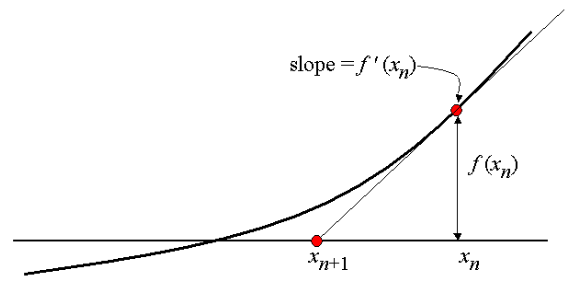
\includegraphics[width=10cm]{images/Newton_Geo.png}
        \end{center}
        \caption{Biểu diễn hình học phương pháp Newton-Raphson}
\end{figure}\\
\hspace*{0.5cm} {Ta vẽ một đường tiếp tuyến với đồ thị $f(x)$ tại điểm $x=x_n$. Đường thẳng này có hệ số góc $f'(x_n)$ và đi qua điểm $(x_n, f(x_n)$ nên có phương trình $y = f'(x_n)(x - x_n) + f(x_n)$. Bây giờ ta tìm nghiệm xấp xỉ mới $x_{n+1}$ của phương trình này. Giải phương trình ta được $x_{n+1} = x_n - \frac{f(x_n)}{f'(x_n)}$}.
\hspace*{0.5cm} {Tuy nhiên phương pháp Newton - Raphson cũng có những giới hạn nhất định. Phương pháp này có thể không hoạt động nếu có các điểm uốn, điểm cực đại hoặc cực tiểu địa phương xung quanh điểm làm gốc $x_0$.}\\
\hspace*{0.5cm} {Phương pháp Newton - Raphson cũng có thể được mở rộng cho hệ phương trình. Cụ thể, đối với hệ phương trình vi phân tổng quát của bài tập này, công thức hồi quy của phương pháp Newton - Raphson sẽ có dạng:}\\
\centerline{$\begin{bmatrix}
    R_{new} \\
    J_{new}
\end{bmatrix} = \begin{bmatrix}
    R_{old} \\
    J_{old}
\end{bmatrix} - \alpha.\begin{bmatrix}
    \frac{\partial f}{\partial R} & \frac{\partial f}{\partial J}\\
    \frac{\partial g}{\partial R} & \frac{\partial g}{\partial J}
\end{bmatrix}^{-1}\begin{bmatrix}
    f \\
    g
\end{bmatrix}$}\\
Trong công thức trên:
\begin{itemize}
    \item $\begin{bmatrix}
    R_{new} \\
    J_{new}
    \end{bmatrix}$ là các giá trị xấp xỉ mới.
    \item $\begin{bmatrix}
    R_{new} \\
    J_{new}
    \end{bmatrix}$ là các giá trị cũ.
    \item $\begin{bmatrix}
    \frac{\partial f}{\partial R} & \frac{\partial f}{\partial J}\\
    \frac{\partial g}{\partial R} & \frac{\partial g}{\partial J}
    \end{bmatrix}$ là ma trận Jacobian: Ma trận Jacobian là ma trận chứa các đạo hàm riêng bậc nhất của các hàm $f, g$ theo các biến $R, J$.
    \item $\begin{bmatrix}
    f \\
    g
    \end{bmatrix}$ là các hàm $f, g$ trong hệ phương trình vi phân.
    \item $\alpha$ là một hệ số chọn. Trong 5 ví dụ bên dưới, ta chọn $\alpha = 1$. 
\end{itemize}
\hspace*{0.5cm}{Giá trị đầu vào cho công thức hồi quy phải ở dạng phương trình Euler ẩn, với các biến, các hàm được định nghĩa như phía dưới:}
\begin{align*}
    R_{k+1} = R_k + f(t_{k+1}, R_{k+1}, J_{k+1}) * h\\
    J_{k+1} = J_k + g(t_{k+1}, R_{k+1}, J_{k+1}) * h
\end{align*}
\hspace*{0.5cm}{Ta đưa hai phương trình trên về dạng sau để áp dụng giải thuật Newton - Raphson:}
\begin{align*}
    R_k + f(t_{k+1}, R_{k+1}, J_{k+1}) * h - R_{k+1} = 0\\
    J_k + g(t_{k+1}, R_{k+1}, J_{k+1}) * h - J{k+1} = 0
\end{align*}
\subsubsection{Nguồn gốc}
\hspace*{0.5cm} {Lấy tích phân phương trình vi phân từ $t_k$ tới $t_k + h$ và áp dụng các định lí cơ bản của tích phân và vi phân để có được:}\\
\hspace*{4cm} {$R(t_k + h) - R(t_k) = \displaystyle\int\limits_{t_k}^{t_k + h}f(
t, R(t), J(t)\;\mathrm{d}t$}\\
\hspace*{0.5cm} {Tính xấp xỉ tích phân trên bằng tổng Riemann phải, ta được:}\\
\hspace*{4cm} {$\displaystyle\int\limits_{t_k}^{t_k + h}f(t, R(t), J(t)\;\mathrm{d}t \approx hf(t_{k+1}, R(t_{k+1}), J(t_{k+1})$}\\
\hspace*{0.5cm} {Kết hợp cả 2 phương trình, ta suy ra phương pháp Euler ẩn. Chứng minh tương tự với hàm $J(t)$.}
\subsubsection{Sai số cắt ngắn cục bộ}
\hspace*{0.5cm} {Giống với phương pháp Euler tường minh, sai số cắt ngắn cục bộ của phương pháp Euler ẩn cũng được tính theo công thức:}\\
\hspace*{4cm} {$E(t_1) = \sqrt{[R(t_1) - R_1]^2 + [J(t_1) - J_1]^2}$}\\
\hspace*{0.5cm} {Với $t_0 = t_1 - h$, áp dụng khai triển Taylor đối với $R(t_0)$ và $J(t_0)$, ta có:}
\begin{align}
    \begin{cases}
        R(t_0) = R(t_1 - h) = R(t_1) - h.R'(t_1) + \frac{1}{2}h^2R"(t_1) + O(h^2)\\
        J(t_0) = J(t_1 - h) = J(t_1) - h.J'(t_1) + \frac{1}{2}h^2J"(t_1) + O(h^2)
    \end{cases}
\end{align}
\begin{align}
    \Rightarrow
    \begin{cases}
        R_0 = R(t_1) - h.f(t_1, R_1, J_1) + \frac{1}{2}h^2f'(t_1, R_1, J_1) + O(h^2)\\
        J_0 = J(t_1) - h.g(t_1, R_1, J_1) + \frac{1}{2}h^2g'(t_1, R_1, J_1) + O(h^2)
    \end{cases}
\end{align}
\begin{align}
    \Rightarrow
    \begin{cases}
        R(t_1) = R_1 - \frac{1}{2}h^2f'(t_1, R_1, J_1) + O(h^2)\\
        J(t_1) = J_1 - \frac{1}{2}h^2g'(t_1, R_1, J_1) + O(h^2)
    \end{cases}
\end{align}
\begin{align}
    \Rightarrow
    \begin{cases}
        R(t_1) - R_1 = -\frac{1}{2}h^2f'(t_1, R_1, J_1) + O(h^2)\\
        J(t_1) - J_1 = -\frac{1}{2}h^2g'(t_1, R_1, J_1) + O(h^2)
    \end{cases}
\end{align}
\hspace*{0.5cm} {Bỏ qua phần $O(h^2)$ ta được:}
\begin{align}
    \begin{cases}
        R(t_1) - R_1 = -\frac{1}{2}h^2f'(t_1, R_1, J_1)\\
        J(t_1) - J_1 = -\frac{1}{2}h^2g'(t_1, R_1, J_1)
    \end{cases}
\end{align}
\hspace*{3cm} {$\Rightarrow E(t_1) \approx \sqrt{[-\frac{1}{2}h^2f'(t_1, R_1, J_1)]^2 + [-\frac{1}{2}h^2g'(t_1, R_1, J_1)]^2}$}\\
\hspace*{4cm} {$= \frac{1}{2}h^2\sqrt{f'^2(t_1,R_1,J_1) + g'^2(t_1,R_1,J_1)}$}\\
\hspace*{0.5cm} {Như vậy, trong phương pháp Euler ẩn, $E(t_1)$ cũng xấp xỉ tỉ lệ thuận với $h^2$.}
\subsubsection{Nhược điểm của phương pháp Euler ẩn}
\hspace*{0.5cm} {Thứ nhất, do trong công thức của phương pháp Euler ẩn có ẩn số $R_{k+1}$ và $J_{k+1}$ ở cả 2 vế của hệ phương trình, nên để tìm được chúng, ta phải giải hệ phương trình đó. Quá trình này có thể tốn nhiều thời gian và phức tạp hơn so với phương pháp Euler tường minh.}\\
\hspace*{0.5cm} {Thứ hai, sai số cắt ngắn cục bộ tỉ lệ thuận với $h^2$, điều này đồng nghĩa với việc khi $h > 1$ sai số sẽ trở nên rất lớn, khi đó khoảng cách giữa nghiệm chính xác và nghiệm gần đúng sẽ là rất lớn, ảnh hưởng tới tính đúng đắn của bài toán}
\subsubsection{Ví dụ}
\textbf{Ví dụ 1:} Tìm nghiệm xấp xỉ của hệ phương trình bằng phương pháp Euler ẩn:
\begin{align*}
    \begin{cases}
        R'=-R+J+\frac{sin(t+1)}{t+1}\\
        J'=-R+J+t \\
        R(0)=2, J(0)=3
    \end{cases}
\end{align*}
\centerline{\textbf{Giải}}\\
Đây là ví dụ về hệ phương trình vi phân tuyến tính không thuần nhất không thể tìm nghiệm chính xác với điều kiện ban đầu $R_0=2, J_0=3$.\\
Công thức hồi quy như sau:
\begin{align*}
    \begin{cases}
        R_n=R_{n-1}+h(-R_n+J_n+\frac{sin(t_n+1)}{t_n+1})\\
        J_n=J_{n-1}+h(-R_n+J_n+t_n)\\
        t_n=t_{n-1}+h
    \end{cases}
\end{align*}
\begin{enumerate}
    \item \textbf{Vẽ đồ thị nghiệm.}\\
    Biểu diễn $R$ và $J$ trên cùng một đồ thị theo biến thời gian $t$ (hình 25):
    \begin{figure}[h!]
        \begin{center}
        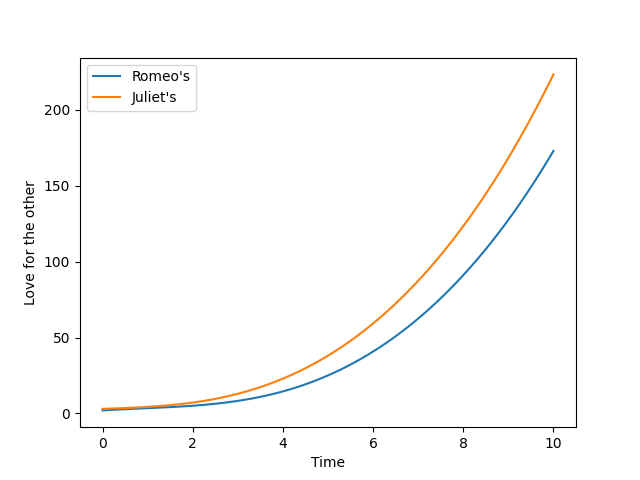
\includegraphics[width=10cm]{images/euler_1.png}
        \end{center}
        \caption{Solution figure Ví dụ 1}
    \end{figure}\\
    Giải thích các đoạn code trong Python vẽ đồ thị ví dụ trên (các đoạn code này được ta định nghĩa trong file \textbf{implicit\_euler\_trajectory.py} và sẽ được dùng để vẽ \textbf{phase portrait}) như sau:
    \begin{itemize}
        \item Nạp các modules cần thiết, bao gồm: \textbf{matplotlib.pyplot}(module đồ họa vẽ đồ thị), \textbf{numpy}(module toán học xử lý ma trận và mảng), \textbf{numpy.linalg.inv}(module để nghịch đảo ma trận), \textbf{math}(hình 26).
        \begin{figure}[h!]
            \begin{center}
            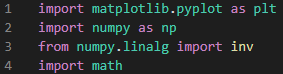
\includegraphics[width=5cm]{images/euler_modules.png}
            \end{center}
            \caption{Nạp modules}
        \end{figure}
        \item Tạo 3 công thức của phương pháp Euler ẩn dưới dạng \textbf{Newton-Raphson} tương ứng với $R$ (Romeo), $J$ (Juliet), $t$ (Thời điểm) (Ở đây, ta tạo thêm một công thức Euler ẩn so với kiến thức chuẩn bị cho biến thời gian $t$ với \textbf{time step = h})(hình 27):
        \begin{center}
            \textbf{\textit{old\_value + h * f(new\_value) - new\_value}}
        \end{center}
         \begin{figure}[h!]
            \begin{center}
            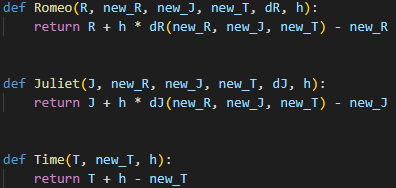
\includegraphics[width=8cm]{images/euler_func.png}
            \end{center}
            \caption{Công thức Euler ẩn của \textbf{Romeo, Juliet, Time}}
        \end{figure}
        \item Tạo ma trận \textbf{Jacobian} để tính toán đạo hàm riêng theo từng biến của 3 công thức Euler ẩn của hệ phương trình vi phân đa biến (Ma trận \textbf{Jacobian} bao gồm 9 hạng tử) (hình 28).
         \begin{figure}[h!]
            \begin{center}
            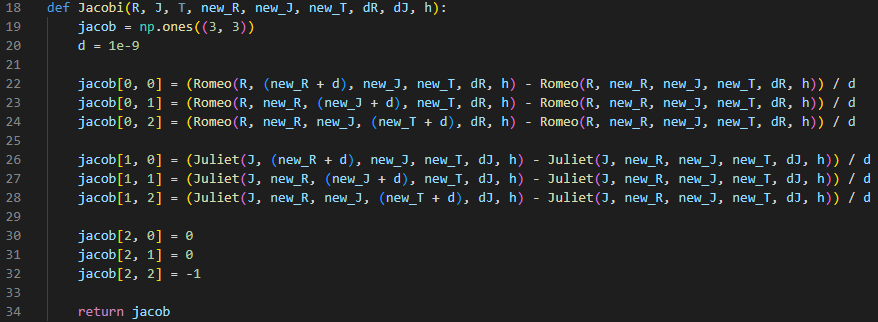
\includegraphics[width=12cm]{images/jacobi.png}
            \end{center}
            \caption{Ma trận Jacobian}
        \end{figure}
        \item Viết thuật toán \textbf{Newton-Raphson}, vòng lặp của thuật toán \textbf{Newton-Raphson} dừng lại khi sai số cắt ngắn cục bộ \textbf{LTE} có thể chấp nhận được (cụ thể $error < 10^{-9}$) tại một thời điểm $t$ (hình 29).
         \begin{figure}[h!]
            \begin{center}
            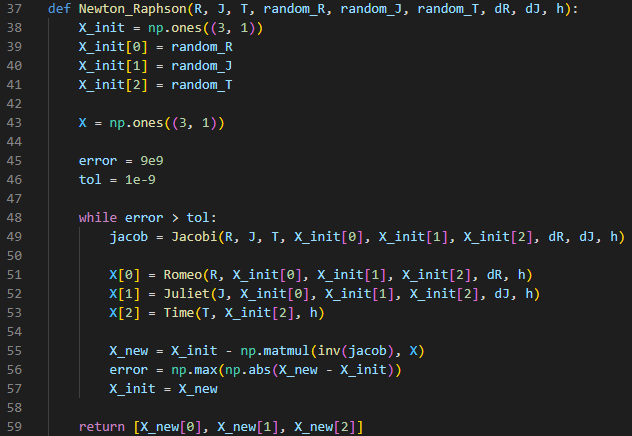
\includegraphics[width=10cm]{images/Newton_Raphson.png}
            \end{center}
            \caption{Giải thuật \textbf{Newton-Raphson}}
        \end{figure}
        \item Viết hàm \textbf{implicit\_euler} theo phương pháp Euler ẩn sử dụng giải thuật \textbf{Newton-Raphson} để tính toán nghiệm xấp xỉ cho hệ phương trình vi phân (hình 30).
         \begin{figure}[h!]
            \begin{center}
            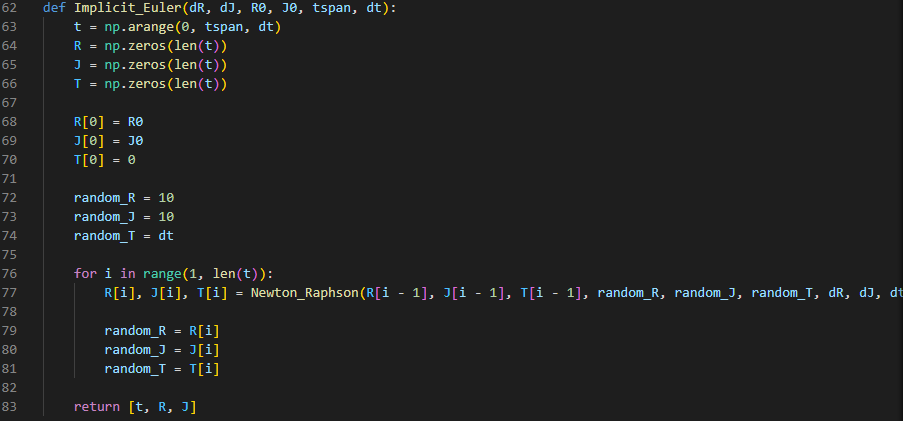
\includegraphics[width=14cm]{images/implicit_euler.png}
            \end{center}
            \caption{Phương pháp Euler ẩn}
        \end{figure}
        \item Cuối cùng ta nhập các công thức của $R', J'$, các giá trị ban đầu $R_0, J_0$ đã cho trong hệ phương trình vi phân. Chọn bước nhảy thời gian \textbf{time step} $h = 0.001$ và sau đó vẽ hình (hình 31).
        \begin{figure}[h!]
            \begin{center}
            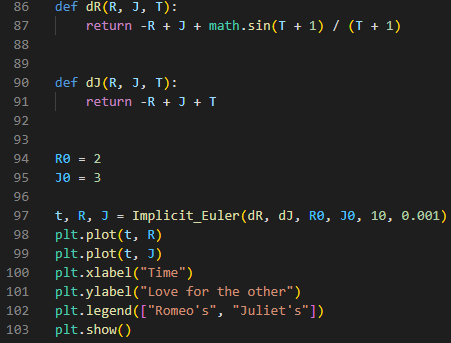
\includegraphics[width=8cm]{images/euler_plot.png}
            \end{center}
            \caption{Nhập input và xuất ra output}
        \end{figure}
    \end{itemize}
    \item \textbf{Vẽ Phase portrait}\\
    Phase portrait của hệ phương trình vi phân
    \begin{align*}
        \begin{cases}
            R'=-R+J+\frac{sin(t+1)}{t+1}\\
            J'=-R+J+t
        \end{cases}
    \end{align*}
    với điều kiện ban đầu bất kì trong mặt phẳng $RJ$ được biểu diễn trong hình 32.
    \begin{figure}[h!]
        \begin{center}
        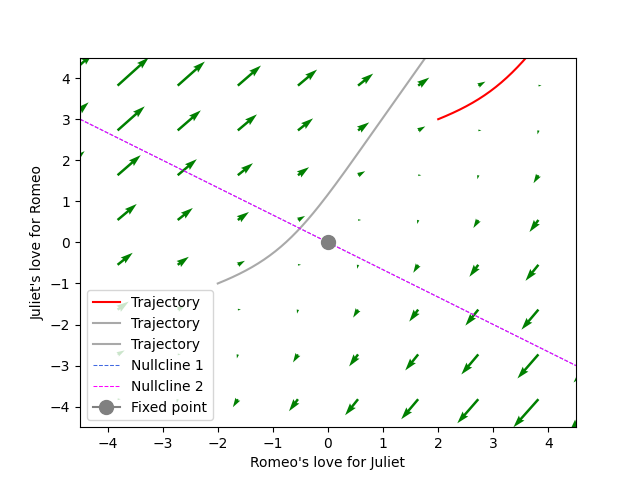
\includegraphics[width=10cm]{images/euler_1_portrait.png}
        \end{center}
        \caption{Phase portrait figure}
    \end{figure}\\
    Đoạn code Python được sử dụng để vẽ phase portrait tương tự như \textbf{Bài tập 2}:
    \begin{lstlisting}
        import numpy as np
        import matplotlib.pyplot as plt
        from scipy.integrate import odeint
        from implicit_euler_trajectory import dR, dJ, R0, J0
        Sts = [[R0, J0], [R0 + 4, J0 + 4], [R0 - 4, J0 - 4]]
        # ODE System
        
        
        def ivpSys(s, t, dR, dJ):
            R, J = s
            T = t
            dRdt = dR(R, J, T)
            dJdt = dJ(R, J, T)
            return [dRdt, dJdt]
        
        
        # Vector R', J' at t = 0 with 144 values of pair (R0, J0)
        y1 = np.linspace(-6, 6, 12)
        y2 = np.linspace(-6, 6, 12)
        Y1, Y2 = np.meshgrid(y1, y2)
        t = 0
        u, v = np.zeros(Y1.shape), np.zeros(Y2.shape)
        NI, NJ = Y1.shape
        for i in range(NI):
            for j in range(NJ):
                x = Y1[i, j]
                y = Y2[i, j]
                yvector = ivpSys([x, y], t, dR, dJ)
                u[i, j] = yvector[0]
                v[i, j] = yvector[1]
        Q = plt.quiver(Y1, Y2, u, v, color='g')
        # Trajectory of Sts with 200 values of t between (0,5)
        tspan = np.linspace(0, 5, 200)
        for elementSt, St in enumerate(Sts):
            sol = odeint(ivpSys, St, tspan, args=(dR, dJ))
            if elementSt == 0:
                color = "r"
            else:
                color = "darkgray"
            plt.plot(sol[:, 0], sol[:, 1], color, label='Trajectory')
        # Figure phase portrait
        x = np.linspace(-4.5, 4.5, 100)
        
        
        def fx(x, a, b):
            return -a * x / b
        
        
        plt.plot(x, fx(x, 2, 3), linestyle='dashed', linewidth=0.75,
                 color='royalblue', label='Nullcline 1')
        plt.plot(x, fx(x, 2, 3), linestyle='dashed', linewidth=0.75,
                 color='magenta', label='Nullcline 2')
        plt.plot(0, 0, "red", marker="o", markersize=10.0,
                 color='grey', label='Fixed point')
        plt.xlabel("Romeo's love for Juliet")
        plt.ylabel("Juliet's love for Romeo")
        plt.legend()
        plt.xlim([-4.5, 4.5])
        plt.ylim([-4.5, 4.5])
        plt.show()
    \end{lstlisting}
\end{enumerate}
\textbf{Ví dụ 2:}  Tìm nghiệm xấp xỉ của hệ phương trình bằng phương pháp Euler ẩn:
\begin{align*}
    \begin{cases}
        R'=R(1 - J) \\
        J'=R(1 - J) \\
        R(0)=2, J(0)=3
    \end{cases}
\end{align*}
\centerline{\textbf{Giải}}\\
Đây là ví dụ về hệ phương trình vi phân thường cấp 1 tổng quát không thể tìm nghiệm chính xác với điều kiện ban đầu $R0=2, J0=3$.\\
Công thức hồi quy như sau:
\begin{align*}
    \begin{cases}
        R_n=R_{n-1}+h(R_n - R_n * J_n)\\
        J_n=J_{n-1}+h(R_n - R_n * J_n)\\
        T_n=T_{n-1}+h
    \end{cases}
\end{align*}
Chọn $h=0.001$. Đoạn code trong Python dùng để vẽ đồ thị và phase portrait tương tự như \textbf{ví dụ 1}, chỉ thay đổi $dR, dJ, R0, J0$. Hình vẽ được biểu diễn ở hình 33.
\begin{figure}[h!]
    \begin{center}
        \begin{tabular}{cc}
             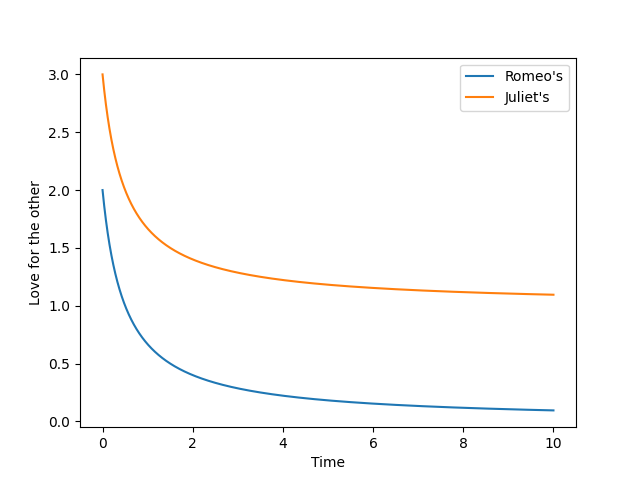
\includegraphics[width=7cm]{images/euler_2.png} &
             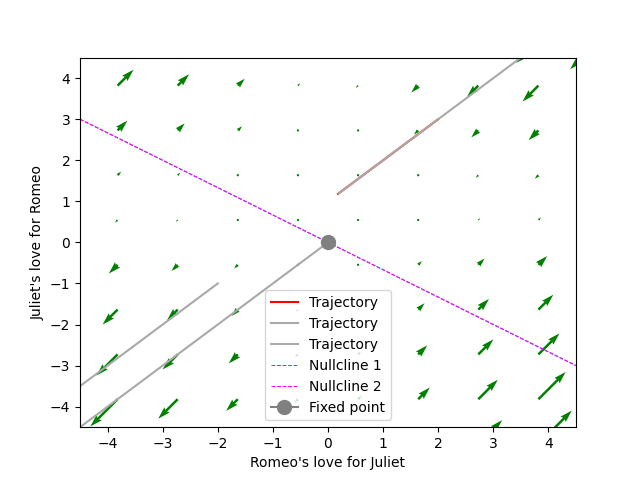
\includegraphics[width=7cm]{images/euler_2_portrait.png}\\
        \end{tabular}
        \caption{Solution figure và phase portrait figure Ví dụ 2}
    \end{center}
\end{figure}\\
\textbf{Ví dụ 3:}  Tìm nghiệm xấp xỉ của hệ phương trình bằng phương pháp Euler ẩn:
\begin{align*}
    \begin{cases}
        R'=-3R+4J+sin(t)\\
        J'=-2R+3J+t\\
        R(0)=0, J(0)=1
    \end{cases}
\end{align*}
\centerline{\textbf{Giải}}\\
Đây là ví dụ về hệ phương trình vi phân tuyến tính không thuần nhất với hệ số không đổi và giá trị ban đầu $R0 = 0, J0 = 1$.\\
Công thức hồi quy như sau:
\begin{align*}
    \begin{cases}
        R_n=R_{n-1}+h(-3R_n+4J_n+\sin(T_n))\\
        J_n=J_{n-1}+h(-2R_n+3J_n+T_n)\\
        T_n=T_{n-1}+h
    \end{cases}
\end{align*}
Chọn $h=0.001$. Đoạn code trong Python dùng để vẽ đồ thị và phase portrait tương tự như \textbf{ví dụ 1}, chỉ thay đổi $dR, dJ, R0, J0$. Hình vẽ được biểu diễn ở hình 34.
\begin{figure}[h!]
    \begin{center}
        \begin{tabular}{cc}
             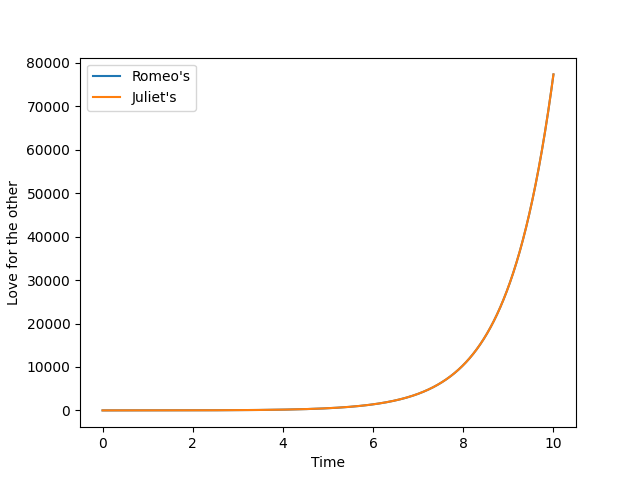
\includegraphics[width=7cm]{images/euler_3.png} &
             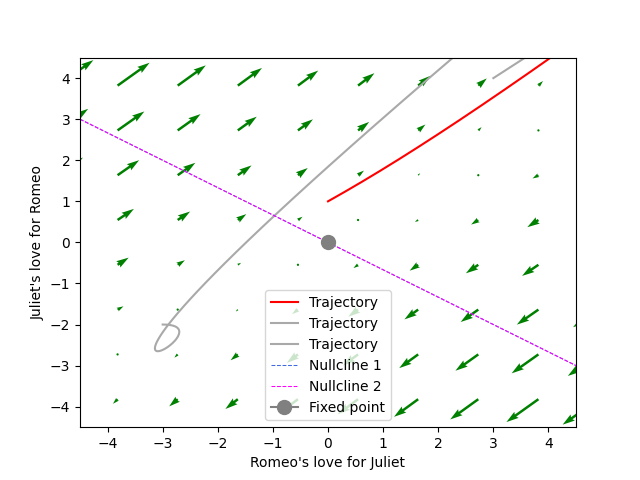
\includegraphics[width=7cm]{images/euler_3_portrait.png}\\
        \end{tabular}
        \caption{Solution figure và phase portrait figure Ví dụ 3}
    \end{center}
\end{figure}\\
\textbf{Ví dụ 4:}  Tìm nghiệm xấp xỉ của hệ phương trình bằng phương pháp Euler ẩn:
\begin{align*}
    \begin{cases}
        R'=J+t-1\\
        J'=-R+t^2\\
        R(0)=1, J(0)=2
    \end{cases}
\end{align*}
\centerline{\textbf{Giải}}\\
Đây là ví dụ về hệ phương trình vi phân tuyến tính không thuần nhất với hệ số không đổi và giá trị ban đầu $R0 = 1, J0 = 2$.\\
Công thức hồi quy như sau:
\begin{align*}
    \begin{cases}
        R_n=R_{n-1}+h(J_n + T_n - 1)\\
        J_n=J_{n-1}+h(-R_n + T_n^2)\\
        T_n=T_{n-1}+h
    \end{cases}
\end{align*}
Chọn $h=0.001$. Đoạn code trong Python dùng để vẽ đồ thị và phase portrait tương tự như \textbf{ví dụ 1}, chỉ thay đổi $dR, dJ, R0, J0$. Hình vẽ được biểu diễn ở hình 35.
\begin{figure}[h!]
    \begin{center}
        \begin{tabular}{cc}
             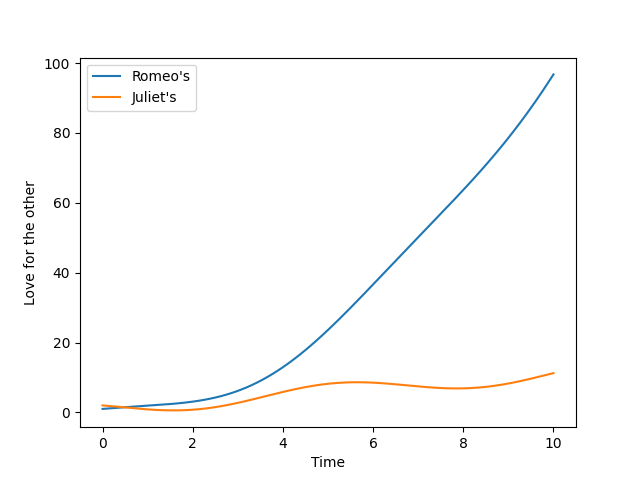
\includegraphics[width=7cm]{images/euler_4.png} &
             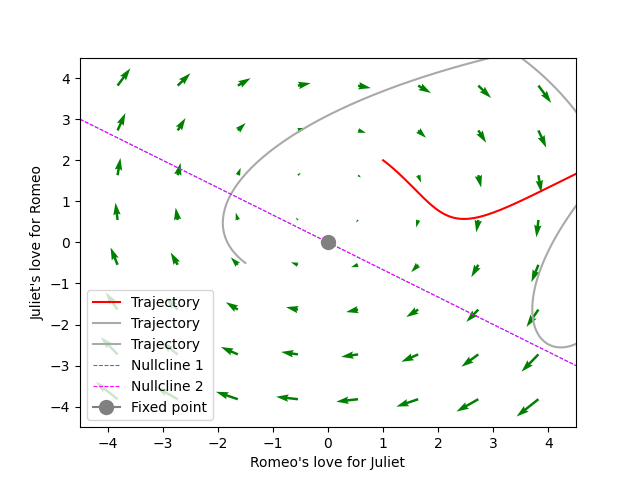
\includegraphics[width=7cm]{images/euler_4_portrait.png}\\
        \end{tabular}
        \caption{Solution figure và phase portrait figure Ví dụ 4}
    \end{center}
\end{figure}\\
\textbf{Ví dụ 5:}  Tìm nghiệm xấp xỉ của hệ phương trình bằng phương pháp Euler ẩn:
\begin{align*}
    \begin{cases}
        R'=-4R + RJ\\
        J'=R^2 - 3J\\
        R(0)=2, J(0)=3
    \end{cases}
\end{align*}
\centerline{\textbf{Giải}}\\
Đây là ví dụ về hệ phương trình vi phân thường cấp 1 tổng quát không thể tìm nghiệm chính xác với điều kiện ban đầu $R0 = 2, J0 = 3$.\\
Công thức hồi quy như sau:
\begin{align*}
    \begin{cases}
        R_n=R_{n-1}+h(-4R_n + R_nJ_n)\\
        J_n=J_{n-1}+h(R_n^2 - 3J_n)\\
        T_n=T_{n-1}+h
    \end{cases}
\end{align*}
Chọn $h=0.001$. Đoạn code trong Python dùng để vẽ đồ thị và phase portrait tương tự như \textbf{ví dụ 1}, chỉ thay đổi $dR, dJ, R0, J0$. Hình vẽ được biểu diễn ở hình 36.
\begin{figure}[h!]
    \begin{center}
        \begin{tabular}{cc}
             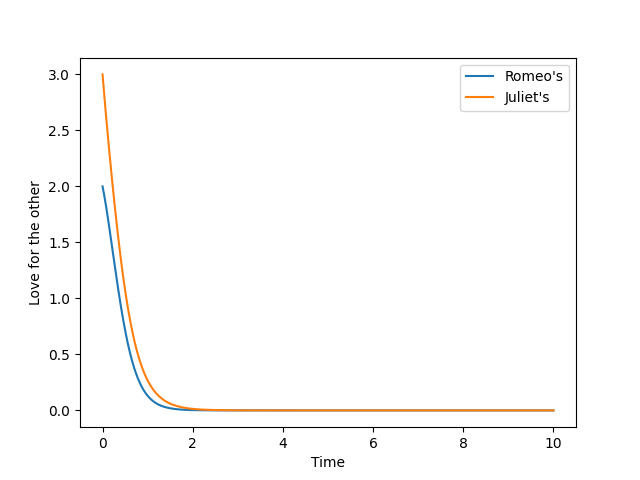
\includegraphics[width=7cm]{images/euler_5.png} &
             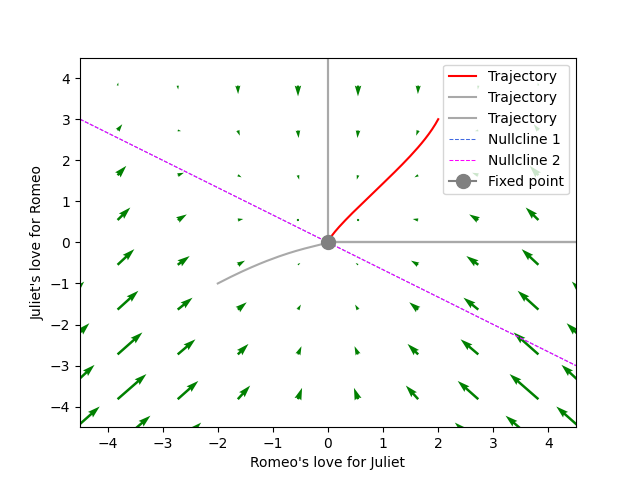
\includegraphics[width=7cm]{images/euler_5_portrait.png}\\
        \end{tabular}
        \caption{Solution figure và phase portrait figure Ví dụ 5}
    \end{center}
\end{figure}\\
\textbf{Link toàn bộ bài làm của nhóm:}\\
\url{https://github.com/ngyngcphu/Dynamics-of-Love}